% Options for packages loaded elsewhere
\PassOptionsToPackage{unicode}{hyperref}
\PassOptionsToPackage{hyphens}{url}
%
\documentclass[
  10pt,
  a4paper,
]{article}
\usepackage{amsmath,amssymb}
\usepackage{lmodern}
\usepackage{iftex}
\ifPDFTeX
  \usepackage[T1]{fontenc}
  \usepackage[utf8]{inputenc}
  \usepackage{textcomp} % provide euro and other symbols
\else % if luatex or xetex
  \usepackage{unicode-math}
  \defaultfontfeatures{Scale=MatchLowercase}
  \defaultfontfeatures[\rmfamily]{Ligatures=TeX,Scale=1}
\fi
% Use upquote if available, for straight quotes in verbatim environments
\IfFileExists{upquote.sty}{\usepackage{upquote}}{}
\IfFileExists{microtype.sty}{% use microtype if available
  \usepackage[]{microtype}
  \UseMicrotypeSet[protrusion]{basicmath} % disable protrusion for tt fonts
}{}
\makeatletter
\@ifundefined{KOMAClassName}{% if non-KOMA class
  \IfFileExists{parskip.sty}{%
    \usepackage{parskip}
  }{% else
    \setlength{\parindent}{0pt}
    \setlength{\parskip}{6pt plus 2pt minus 1pt}}
}{% if KOMA class
  \KOMAoptions{parskip=half}}
\makeatother
\usepackage{xcolor}
\IfFileExists{xurl.sty}{\usepackage{xurl}}{} % add URL line breaks if available
\IfFileExists{bookmark.sty}{\usepackage{bookmark}}{\usepackage{hyperref}}
\hypersetup{
  hidelinks,
  pdfcreator={LaTeX via pandoc}}
\urlstyle{same} % disable monospaced font for URLs
\usepackage[margin=0.8in]{geometry}
\usepackage{longtable,booktabs,array}
\usepackage{calc} % for calculating minipage widths
% Correct order of tables after \paragraph or \subparagraph
\usepackage{etoolbox}
\makeatletter
\patchcmd\longtable{\par}{\if@noskipsec\mbox{}\fi\par}{}{}
\makeatother
% Allow footnotes in longtable head/foot
\IfFileExists{footnotehyper.sty}{\usepackage{footnotehyper}}{\usepackage{footnote}}
\makesavenoteenv{longtable}
\usepackage{graphicx}
\makeatletter
\def\maxwidth{\ifdim\Gin@nat@width>\linewidth\linewidth\else\Gin@nat@width\fi}
\def\maxheight{\ifdim\Gin@nat@height>\textheight\textheight\else\Gin@nat@height\fi}
\makeatother
% Scale images if necessary, so that they will not overflow the page
% margins by default, and it is still possible to overwrite the defaults
% using explicit options in \includegraphics[width, height, ...]{}
\setkeys{Gin}{width=\maxwidth,height=\maxheight,keepaspectratio}
% Set default figure placement to htbp
\makeatletter
\def\fps@figure{htbp}
\makeatother
\setlength{\emergencystretch}{3em} % prevent overfull lines
\providecommand{\tightlist}{%
  \setlength{\itemsep}{0pt}\setlength{\parskip}{0pt}}
\setcounter{secnumdepth}{-\maxdimen} % remove section numbering
\ifLuaTeX
  \usepackage{selnolig}  % disable illegal ligatures
\fi

\author{}
\date{}

\usepackage{titlesec}
\usepackage{fancyhdr}
\definecolor{reportnavy}{HTML}{17324D}
\definecolor{reportteal}{HTML}{147D83}
\titleformat{\section}{\Large\bfseries\color{reportnavy}}{}{0pt}{}
\titleformat{\subsection}{\large\bfseries\color{reportteal}}{}{0pt}{}
\pagestyle{fancy}\fancyhf{}
\fancyhead[L]{\small Computer Networks | Phase 3 CPU Extension}
\fancyfoot[L]{\small 23I-2568 | 23I-2581}
\fancyfoot[R]{\small\thepage}
\setlength{\headheight}{15pt}
\setlength{\emergencystretch}{3em}

\begin{document}

\hypertarget{phase-3-prospective-cpu-extension}{%
\section{Phase 3: Prospective CPU
Extension}\label{phase-3-prospective-cpu-extension}}

Saneedullah (23I-2568) and Ahmed Bilal (23I-2581) \textbar{} 16 November
2026

\hypertarget{status-and-scope}{%
\subsection{Status and scope}\label{status-and-scope}}

This appendix supplements the preceding report. It contains 273
completed full trajectories and 24 paired oracle suffixes from a
separately frozen CPU protocol. Core status: \textbf{complete (240
trajectories, twelve ownership seeds)}. The original 696 GPU and 57 CPU
results remain distinct historical experiments. These counts must not be
pooled as independent replicates.

The new experiment restores the Phase 2 single-attacker design, twelve
independent ownership/randomization seeds, client-local importance and
the exact label-repair intervention. It uses the previously selected
reference-engine clean parameters, with a fresh clean feasibility check
before primary runs. \textbf{All outcomes in this appendix use the
frozen development bank, not an independent final-test bank.} Historical
use of that bank for model selection limits generalization claims;
prospective randomization does not turn it into a new final test.

\hypertarget{reproducible-implementation-and-clean-feasibility}{%
\subsection{Reproducible implementation and clean
feasibility}\label{reproducible-implementation-and-clean-feasibility}}

Python 3.12.14, PyTorch 2.7.0+cpu, NumPy 2.3.5; CPU FP32, deterministic
operations, two worker processes and one numerical thread per worker.
Four stages, five persistent clients, 12 rounds per stage, one local
epoch, batch 128, Adam learning rate .001. EI uses client-local
per-example empirical importance (coefficient 100); replay uses 500
records per client, supervised replay coefficient 1 and dark-logit
coefficient .1. Newly introduced head rows use Xavier initialization. DC
and DM admit equal totals per client, using q=.75 and rare floor20.
Attack ownership is whole-component Dirichlet(.5); one eligible client
receives E2-only Hulk-to-benign corruption at nested doses 0, .1, .3 and
.5. No escalation is selected from observed effects. The fixed benign
bank is present at every stage.

Clean-gate outcome: \textbf{passed}. All nine clean final model hashes
also reproduce the corresponding historical selected reference-engine
runs exactly. Each learner must average at least .5 E1 recall on both
FTP and SSH and .7 E2 Hulk recall across development ownership seeds
101--103. New ownership seeds are 1--11 and 42. They quantify variation
within this historical capture, not across independent organizations,
campaigns or days. The gate is an average over three partitions; passing
it does not establish that every partition learned each family. Per-seed
gate recalls are retained in clean-gates.json.

\begin{longtable}[]{@{}llllll@{}}
\toprule
learner & stage & code & mean\_recall & threshold & passed \\
\midrule
\endhead
FT & 1 & 7 & 0.6667 & 0.5000 & True \\
FT & 1 & 12 & 0.9972 & 0.5000 & True \\
FT & 2 & 4 & 0.9997 & 0.7000 & True \\
EI & 1 & 7 & 0.6667 & 0.5000 & True \\
EI & 1 & 12 & 0.9972 & 0.5000 & True \\
EI & 2 & 4 & 0.9997 & 0.7000 & True \\
DR & 1 & 7 & 0.6667 & 0.5000 & True \\
DR & 1 & 12 & 0.9983 & 0.5000 & True \\
DR & 2 & 4 & 0.9998 & 0.7000 & True \\
\bottomrule
\end{longtable}

\hypertarget{primary-outcomes}{%
\subsection{Primary outcomes}\label{primary-outcomes}}

H is the E3/E4 mean change in Hulk-to-benign error relative to the same
method's clean trajectory. Negative values favor the poisoned run on
this endpoint and are reported without clipping. A equally weights
stages E2--E4, then eligible newly introduced untargeted families within
each stage. Macro F1 restricts the true-label population to eligible
seen classes while retaining all prediction columns. Binary metrics and
per-stage matrices are supplied in machine-readable files.

\begin{longtable}[]{@{}llllll@{}}
\toprule
method & dose & macro\_f1 & H & A & benign\_far \\
\midrule
\endhead
DC & 0.0000 & 0.5047 & 0.0000 & 0.2957 & 0.1137 \\
DC & 0.1000 & 0.5088 & -0.0000 & 0.2898 & 0.1292 \\
DC & 0.3000 & 0.5084 & 0.0001 & 0.2820 & 0.1271 \\
DC & 0.5000 & 0.4943 & 0.0003 & 0.2867 & 0.1311 \\
DM & 0.0000 & 0.5892 & 0.0000 & 0.3988 & 0.0561 \\
DM & 0.1000 & 0.5953 & 0.0004 & 0.4017 & 0.0569 \\
DM & 0.3000 & 0.6070 & 0.0031 & 0.3926 & 0.0575 \\
DM & 0.5000 & 0.5910 & 0.0112 & 0.3845 & 0.0560 \\
DR & 0.0000 & 0.6272 & 0.0000 & 0.3897 & 0.0631 \\
DR & 0.1000 & 0.6258 & 0.0003 & 0.3883 & 0.0615 \\
DR & 0.3000 & 0.6299 & 0.0020 & 0.3888 & 0.0597 \\
DR & 0.5000 & 0.6257 & 0.0087 & 0.3883 & 0.0604 \\
EI & 0.0000 & 0.1113 & 0.0000 & 0.2140 & 0.3626 \\
EI & 0.1000 & 0.1066 & 0.0474 & 0.2131 & 0.4218 \\
EI & 0.3000 & 0.1122 & 0.0754 & 0.2063 & 0.3798 \\
EI & 0.5000 & 0.1105 & 0.0882 & 0.2161 & 0.3920 \\
FT & 0.0000 & 0.1063 & 0.0000 & 0.2516 & 0.4420 \\
FT & 0.1000 & 0.1020 & 0.1202 & 0.2681 & 0.4757 \\
FT & 0.3000 & 0.0970 & 0.1334 & 0.2701 & 0.5203 \\
FT & 0.5000 & 0.1030 & 0.1397 & 0.2711 & 0.4707 \\
\bottomrule
\end{longtable}

At dose .5, DC has lower mean untargeted acquisition than DM (A
difference -0.0977) and lower mean poisoning-associated persistence (H
difference -0.0109). These are distinct endpoints: protecting
new-labelled admission does not by itself establish resistance to
mislabeled Hulk records. Clean final macro F1 is 0.1063 for FT, 0.1113
for EI and 0.6272 for DR. Interpret these differences with the paired
intervals and the single corrected family below. Neither a favorable
mean nor non-significance establishes universal superiority or
equivalence. The reference engine changes several historical numerical
choices together; this study does not identify the individual causal
benefit of batch size, head initialization or importance handling.

\begin{figure}
\centering
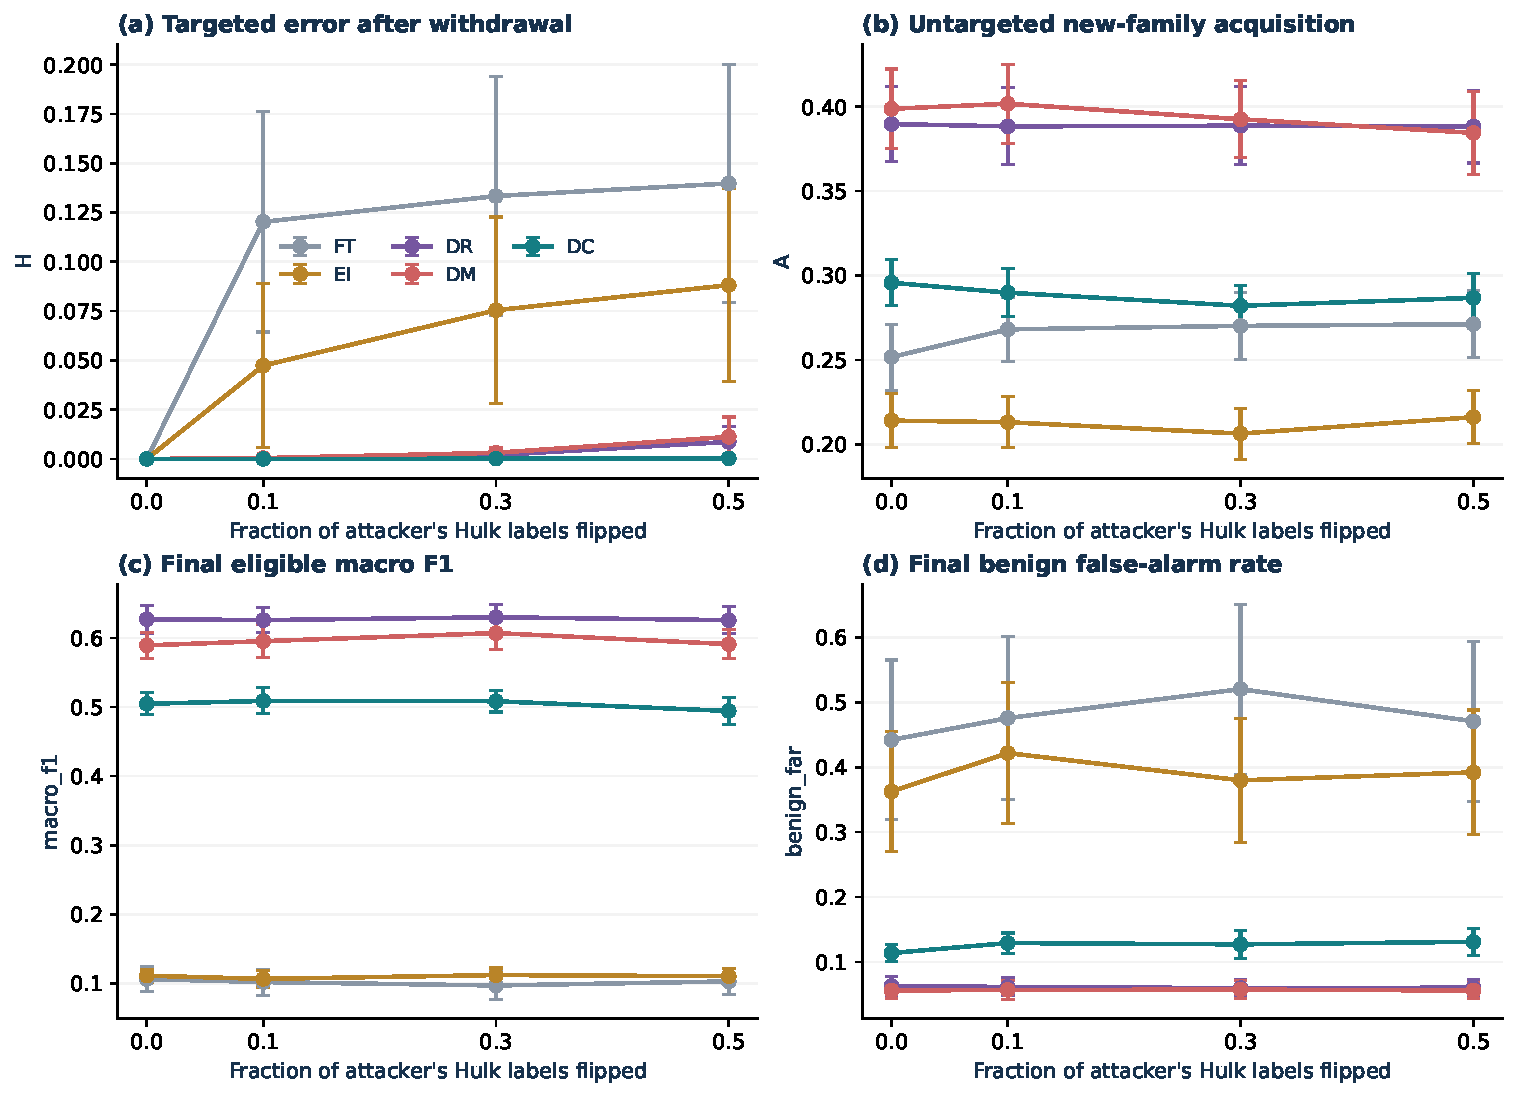
\includegraphics{core-results.pdf}
\caption{Primary results. Points are ownership-seed means; error bars
are standard errors across completed seeds, not uncertainty across
independent captures.}
\end{figure}

The complete trajectory table also reports accuracy, binary
precision/recall/F1, Hulk recall and false-alarm rate. Rare-family
errors remain in each full-inventory 16 by 16 confusion matrix;
unsupported true rows are retained as zero support. Binary metrics are
supplied for both the eligible population and, in separately named
full\_inventory columns, every supported seen family.

\hypertarget{paired-inference-and-uncertainty}{%
\subsection{Paired inference and
uncertainty}\label{paired-inference-and-uncertainty}}

The analysis specification was frozen before the new primary runs. One
family of 29 comparisons follows Phase 2: 18 learner-pair contrasts for
H and immediate Hulk recall change, four DC-minus-DM acquisition
contrasts, six corresponding security contrasts and one clean
false-alarm contrast. Tests use two-sided conditional signed-rank sign
enumeration, averaged tied ranks, zero removal and one Holm correction
across all 29 tests. Bootstrap intervals resample whole paired seeds
10,000 times and are descriptive, not simultaneous. The development-bank
status makes these comparisons exploratory evidence despite their
prospective specification. Non-significance is not equivalence;
seed-level intervals are not capture-level intervals.

\begin{longtable}[]{@{}lllllll@{}}
\toprule
endpoint & contrast & dose & mean & ci\_low & ci\_high & holm\_p \\
\midrule
\endhead
H & FT - EI & 0.1000 & 0.0729 & 0.0006 & 0.1728 & 1.0000 \\
H & FT - EI & 0.3000 & 0.0580 & 0.0040 & 0.1434 & 1.0000 \\
H & FT - EI & 0.5000 & 0.0515 & -0.0092 & 0.1367 & 0.7178 \\
H & FT - DR & 0.1000 & 0.1200 & 0.0162 & 0.2300 & 0.0254 \\
H & FT - DR & 0.3000 & 0.1314 & 0.0212 & 0.2501 & 0.7178 \\
H & FT - DR & 0.5000 & 0.1311 & 0.0214 & 0.2546 & 0.2808 \\
H & EI - DR & 0.1000 & 0.0471 & -0.0052 & 0.1342 & 1.0000 \\
H & EI - DR & 0.3000 & 0.0734 & -0.0028 & 0.1720 & 1.0000 \\
H & EI - DR & 0.5000 & 0.0795 & -0.0074 & 0.1840 & 1.0000 \\
delta\_recall & FT - EI & 0.1000 & 0.0000 & -0.0000 & 0.0000 & 1.0000 \\
delta\_recall & FT - EI & 0.3000 & 0.0002 & 0.0000 & 0.0005 & 1.0000 \\
delta\_recall & FT - EI & 0.5000 & 0.0002 & -0.0000 & 0.0005 & 1.0000 \\
delta\_recall & FT - DR & 0.1000 & 0.0000 & -0.0000 & 0.0000 & 1.0000 \\
delta\_recall & FT - DR & 0.3000 & 0.0000 & -0.0000 & 0.0000 & 1.0000 \\
delta\_recall & FT - DR & 0.5000 & 0.0006 & -0.0000 & 0.0017 & 1.0000 \\
delta\_recall & EI - DR & 0.1000 & 0.0000 & -0.0000 & 0.0000 & 1.0000 \\
delta\_recall & EI - DR & 0.3000 & -0.0002 & -0.0005 & 0.0000 &
1.0000 \\
delta\_recall & EI - DR & 0.5000 & 0.0004 & -0.0005 & 0.0018 & 1.0000 \\
A & DC - DM & 0.0000 & -0.1030 & -0.1284 & -0.0757 & 0.0142 \\
A & DC - DM & 0.1000 & -0.1119 & -0.1475 & -0.0707 & 0.0366 \\
A & DC - DM & 0.3000 & -0.1105 & -0.1419 & -0.0804 & 0.0142 \\
A & DC - DM & 0.5000 & -0.0977 & -0.1367 & -0.0497 & 0.1641 \\
H & DC - DM & 0.1000 & -0.0005 & -0.0013 & -0.0000 & 1.0000 \\
H & DC - DM & 0.3000 & -0.0030 & -0.0086 & -0.0001 & 0.4082 \\
H & DC - DM & 0.5000 & -0.0109 & -0.0308 & -0.0004 & 0.9927 \\
delta\_recall & DC - DM & 0.1000 & 0.0005 & 0.0000 & 0.0013 & 1.0000 \\
delta\_recall & DC - DM & 0.3000 & 0.0046 & -0.0000 & 0.0121 & 1.0000 \\
delta\_recall & DC - DM & 0.5000 & 0.0167 & 0.0000 & 0.0453 & 1.0000 \\
benign\_far & DC - DM & 0.0000 & 0.0576 & 0.0480 & 0.0680 & 0.0142 \\
\bottomrule
\end{longtable}

\hypertarget{exact-replay-label-repair-diagnostic}{%
\subsection{Exact replay label-repair
diagnostic}\label{exact-replay-label-repair-diagnostic}}

At the maximum-dose E2 boundary, DR and DC clone their complete model,
memory and random states. The intervention changes only the replay
labels of poisoned IDs back to Hulk. Features, IDs, cached logits,
widths, occupancy, RNG and weights are unchanged, verified by hashes.
The original branch continues unchanged. This is an explanatory oracle,
not a deployable defense, and does not undo E2 weight damage or poisoned
cached logits. A zero-survivor pair remains in the results.

\begin{longtable}[]{@{}
  >{\raggedright\arraybackslash}p{(\columnwidth - 12\tabcolsep) * \real{0.14}}
  >{\raggedright\arraybackslash}p{(\columnwidth - 12\tabcolsep) * \real{0.14}}
  >{\raggedright\arraybackslash}p{(\columnwidth - 12\tabcolsep) * \real{0.14}}
  >{\raggedright\arraybackslash}p{(\columnwidth - 12\tabcolsep) * \real{0.14}}
  >{\raggedright\arraybackslash}p{(\columnwidth - 12\tabcolsep) * \real{0.14}}
  >{\raggedright\arraybackslash}p{(\columnwidth - 12\tabcolsep) * \real{0.14}}
  >{\raggedright\arraybackslash}p{(\columnwidth - 12\tabcolsep) * \real{0.14}}@{}}
\toprule
method & labels mean & labels SD & ASR effect mean & ASR effect SD & F1
effect mean & F1 effect SD \\
\midrule
\endhead
DC & 131.0000 & 79.8453 & -0.0003 & 0.0009 & -0.0054 & 0.0217 \\
DR & 141.0833 & 84.9582 & -0.0087 & 0.0275 & -0.0032 & 0.0135 \\
\bottomrule
\end{longtable}

Effects are repair minus unchanged continuation; negative ASR effects
indicate less targeted benign prediction after label repair. This
estimates the total downstream intervention effect, including later
admission and weight changes. It does not isolate a direct gradient
pathway or prove labels are the only cause.

\hypertarget{ablations-cost-and-remaining-limitations}{%
\subsection{Ablations, cost and remaining
limitations}\label{ablations-cost-and-remaining-limitations}}

Optional complete twelve-seed blocks are reported in
trajectory-metrics.csv with their own block and coefficient/quota
columns. Their scheduling uses runtime only, never favorable outcomes.
See completion.json for completed and omitted blocks.

\begin{longtable}[]{@{}lllllllll@{}}
\toprule
block & method & q & lambda\_y & lambda\_z & dose & macro\_f1 & H & A \\
\midrule
\endhead
matched-random & DQ & 0.7500 & 1.0000 & 0.1000 & 0.0000 & 0.5887 &
0.0000 & 0.3519 \\
matched-random & DQ & 0.7500 & 1.0000 & 0.1000 & 0.5000 & 0.5866 &
0.0008 & 0.3469 \\
\bottomrule
\end{longtable}

Per-seed attacker identity, eligible source count, realized poison count
and global E2 poison share are supplied in realized-attack-doses.csv.
The nominal dose is a fraction of one client's Hulk rows, not of all
clients or all E2 records. Median trajectory wall time was 146.2 s (90th
percentile 172.9 s), including evaluation and checkpointing, measured
under two-process contention. Three clean-reference results include
batch-1 and batch-256 inference median/p95 after ten warm-ups and 100
timed calls. Stage weight file sizes are serialized checkpoint costs,
not measured network traffic.

The stronger CPU design addresses early-learning feasibility,
client-local importance, the prescribed single attacker, partition
replication and exact memory repair. DG, FIFO/class-balanced eviction,
independent-capture evaluation, a validated IoT schema and actual
distributed networking remain outside this extension unless separately
evidenced. No generated result is substituted for missing classroom
feedback. The final-test bank remains sealed. Attack strength may
legitimately be weak under a single-client threat model; null and
adverse results remain valid.

\hypertarget{evidence-and-reproduction}{%
\subsection{Evidence and reproduction}\label{evidence-and-reproduction}}

The package includes source/input/runtime identities, the frozen
analysis, the whole-component ownership source, raw stage confusion
matrices, selected stage weights and per-seed CSVs. SHA-256 validation
covers every packaged file. The reference definitions and literature
context are those in the preceding report; this appendix introduces no
new external performance claims.

Run \texttt{python\ scripts/finalize\_phase3\_overnight.py} to
regenerate this appendix. Use the pinned CPU environment to reproduce
training; original result identities must never be silently pooled with
a different runtime. See docs/phase3-overnight-plan.md and
configs/phase3/overnight-analysis.json.

\end{document}
